\documentclass[tikz,convert={density=300,size=300x300,outfile=\jobname.png}]{standalone}

\usetikzlibrary{automata,calc,trees,positioning,arrows,chains,shapes.geometric,%
decorations.pathreplacing,decorations.pathmorphing,shapes,%
matrix,shapes.symbols,plotmarks,decorations.markings,shadows}

\begin{document}
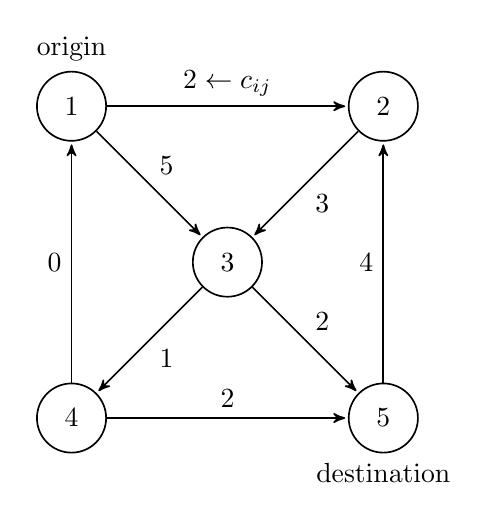
\begin{tikzpicture}[->,>=stealth',shorten >=1pt,auto,node distance=2.8cm,
                    semithick]

  \node[state] (node3) [] {3};
  \node[state] (node1) [above left of=node3, label=above:origin] {1};
  \node[state] (node2) [above right of=node3] {2};
  \node[state] (node4) [below left of=node3] {4};
  \node[state] (node5) [below right of=node3, label=below:destination] {5};

  \path (node1) edge node {$2\leftarrow c_{ij}$} (node2)
        (node1) edge node {5} (node3)
        (node2) edge node {3} (node3)
        (node3) edge node {2} (node5)
        (node3) edge node {1} (node4)
        (node4) edge node {0} (node1)
        (node4) edge node {2} (node5)
        (node5) edge node {4} (node2)
        ;
\end{tikzpicture}
\end{document}